\begin{figure}[!ht]
    \centering
        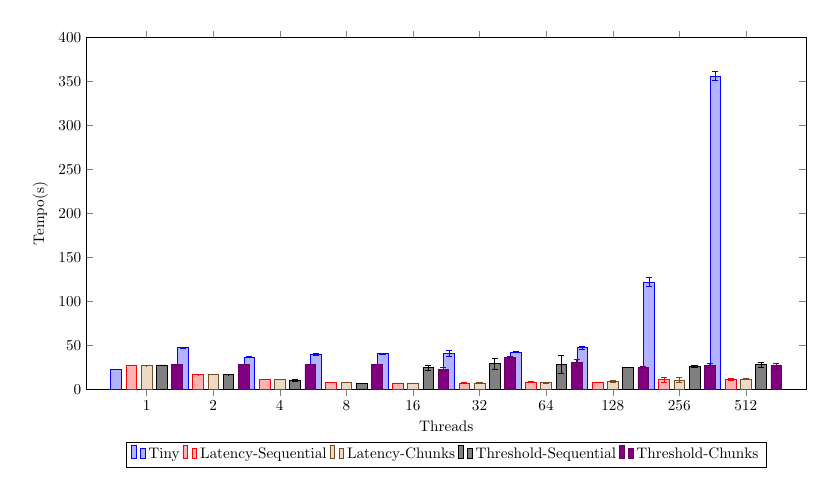
\begin{tikzpicture}[scale=0.55, baseline]
        \begin{axis}[
            width=1.5 \linewidth,
            height=0.8 \linewidth,
            %media de tempo intruder
            ybar=3pt,
            %enlargelimits=0.10,
            legend style={at={(0.5,-0.15)}, anchor=north, legend columns=-1},
            ylabel=Tempo(s),
            xlabel=Threads,
            symbolic x coords={1, 2, 4, 8, 16, 32, 64, 128, 256, 512},
            xtick=data,
            ymin=0,
            ymax=400,
            bar width=7pt,
            % nodes near coords,
            nodes near coords align={vertical},
        ]
        \addplot+[error bars,y dir=both, y explicit] coordinates {
            (1,22.49)+-(1,0.11) (2,47.47)+-(2,0.69) (4,36.62)+-(4,0.59) (8,39.90)+-(8,0.89) (16,40.47)+-(16,0.35) (32,40.54)+-(32,3.55) (64,42.59)+-(64,0.29) (128,47.43)+-(128,1.97) (256,122.18)+-(256,4.64) (512,356.05)+-(512,5.11) 
        };
        \addplot+[error bars,y dir=both, y explicit] coordinates {
            (1,27.06)+-(1,0.18) (2,16.76)+-(2,0.13) (4,11.43)+-(4,0.10) (8,8.18)+-(8,0.13) (16,7.20)+-(16,0.06) (32,7.31)+-(32,0.14) (64,8.25)+-(64,0.81) (128,8.00)+-(128,0.37) (256,10.82)+-(256,3.29) (512,11.20)+-(512,0.86)
        };
        \addplot+[error bars,y dir=both, y explicit] coordinates {
            (1,26.90)+-(1,0.17) (2,16.89)+-(2,0.13) (4,11.50)+-(4,0.13) (8,8.10)+-(8,0.10) (16,7.21)+-(16,0.06) (32,7.28)+-(32,0.07) (64,7.61)+-(64,0.63) (128,9.11)+-(128,0.98) (256,10.40)+-(256,2.68) (512,11.59)+-(512,0.72)
        };
        \addplot+[error bars,y dir=both, y explicit] coordinates {
            (1,27.73)+-(1,0.05) (2,16.65)+-(2,0.16) (4,10.50)+-(4,1.10) (8,6.64)+-(8,0.23) (16,24.42)+-(16,2.56) (32,29.00)+-(32,6.41) (64,28.59)+-(64,10.33) (128,25.01)+-(128,0.29) (256,26.19)+-(256,1.25) (512,27.87)+-(512,2.82)
        };
        \addplot+[error bars,y dir=both, y explicit] coordinates {
            (1,27.96)+-(1,0.25) (2,28.12)+-(2,0.28) (4,28.11)+-(4,0.14) (8,28.17)+-(8,0.07) (16,23.01)+-(16,1.76) (32,36.20)+-(32,1.18) (64,30.24)+-(64,4.39) (128,24.97)+-(128,1.10) (256,26.99)+-(256,2.13) (512,27.18)+-(512,2.84)
        };
        \legend {Tiny, Latency-Sequential, Latency-Chunks, Threshold-Sequential, Threshold-Chunks}
        \end{axis}
        \end{tikzpicture}
    \caption{Tempo de execução em segundos do benchmark Intruder variando o número de \emph{threads}.}
    \label{intruder_tmp}

\end{figure}
